\documentclass[12pt]{article} 
% Custom definitions
% To use this customization file, insert the line "% Custom definitions
% To use this customization file, insert the line "% Custom definitions
% To use this customization file, insert the line "\input{custom}" in the header of the tex file.

% Formatting

\tolerance=1000
\usepackage[margin=1in]{geometry}


% Packages

% \usepackage{amssymb,latexsym}
\usepackage{amssymb,amsfonts,amsmath,latexsym,amsthm}
\usepackage[usenames,dvipsnames]{color}
\usepackage[]{graphicx}
\usepackage[space]{grffile}
\usepackage{mathrsfs}   % fancy math font
% \usepackage[font=small,skip=0pt]{caption}
\usepackage[skip=0pt]{caption}
\usepackage{subcaption}
\usepackage{verbatim}
\usepackage{url}
\usepackage{bm}
\usepackage{dsfont}
\usepackage{extarrows}
\usepackage{multirow}
% \usepackage{wrapfig}
% \usepackage{epstopdf}
\usepackage{rotating}
\usepackage{tikz}
\usetikzlibrary{fit}					% fitting shapes to coordinates
%\usetikzlibrary{backgrounds}	% drawing the background after the foreground

\usepackage{fancyhdr}

\fancypagestyle{firststyle}{
   \fancyhf{}
   \renewcommand{\footrulewidth}{0.4pt}
   \fancyfoot[L]{\footnotesize This work is licensed under a \href{http://creativecommons.org/licenses/by-nc-nd/4.0/}{Creative Commons BY-NC-ND 4.0 International License}.\\ Jeffrey W. Miller (2015). \textit{Lecture Notes on Bayesian Statistics}. Duke University, Durham, NC.}
}


% \usepackage[dvipdfm,colorlinks,citecolor=blue,linkcolor=blue,urlcolor=blue]{hyperref}
\usepackage[colorlinks,citecolor=blue,linkcolor=blue,urlcolor=blue]{hyperref}
%\usepackage{hyperref}
\usepackage[authoryear,round]{natbib}


%  Theorems, etc.

\theoremstyle{plain}
\newtheorem{theorem}{Theorem}[section]
\newtheorem{corollary}[theorem]{Corollary}
\newtheorem{lemma}[theorem]{Lemma}
\newtheorem{proposition}[theorem]{Proposition}
\newtheorem{condition}[theorem]{Condition}
% \newtheorem{conditions}[theorem]{Conditions}

\theoremstyle{definition}
\newtheorem{definition}[theorem]{Definition}
% \newtheorem*{unnumbered-definition}{Definition}
\newtheorem{example}[theorem]{Example}
\theoremstyle{remark}
\newtheorem*{remark}{Remark}
\numberwithin{equation}{section}



% Document-specific shortcuts
\newcommand{\btheta}{{\bm\theta}}
\newcommand{\bbtheta}{{\pmb{\bm\theta}}}

\newcommand{\commentary}[1]{\ifx\showcommentary\undefined\else \emph{#1}\fi}

\newcommand{\term}[1]{\textit{\textbf{#1}}}

% Math shortcuts

% Probability distributions
\DeclareMathOperator*{\Exp}{Exp}
\DeclareMathOperator*{\TExp}{TExp}
\DeclareMathOperator*{\Bernoulli}{Bernoulli}
\DeclareMathOperator*{\Beta}{Beta}
\DeclareMathOperator*{\Ga}{Gamma}
\DeclareMathOperator*{\TGamma}{TGamma}
\DeclareMathOperator*{\Poisson}{Poisson}
\DeclareMathOperator*{\Binomial}{Binomial}
\DeclareMathOperator*{\NormalGamma}{NormalGamma}
\DeclareMathOperator*{\InvGamma}{InvGamma}
\DeclareMathOperator*{\Cauchy}{Cauchy}
\DeclareMathOperator*{\Uniform}{Uniform}
\DeclareMathOperator*{\Gumbel}{Gumbel}
\DeclareMathOperator*{\Pareto}{Pareto}
\DeclareMathOperator*{\Mono}{Mono}
\DeclareMathOperator*{\Geometric}{Geometric}
\DeclareMathOperator*{\Wishart}{Wishart}

% Math operators
\DeclareMathOperator*{\argmin}{arg\,min}
\DeclareMathOperator*{\argmax}{arg\,max}
\DeclareMathOperator*{\Cov}{Cov}
\DeclareMathOperator*{\diag}{diag}
\DeclareMathOperator*{\median}{median}
\DeclareMathOperator*{\Vol}{Vol}

% Math characters
\newcommand{\R}{\mathbb{R}}
\newcommand{\Z}{\mathbb{Z}}
\newcommand{\E}{\mathbb{E}}
\renewcommand{\Pr}{\mathbb{P}}
\newcommand{\I}{\mathds{1}}
\newcommand{\V}{\mathbb{V}}

\newcommand{\A}{\mathcal{A}}
\newcommand{\C}{\mathcal{C}}
\newcommand{\D}{\mathcal{D}}
\newcommand{\Hcal}{\mathcal{H}}
\newcommand{\M}{\mathcal{M}}
\newcommand{\N}{\mathcal{N}}
\newcommand{\X}{\mathcal{X}}
\newcommand{\Zcal}{\mathcal{Z}}
\renewcommand{\P}{\mathcal{P}}

\newcommand{\T}{\mathtt{T}}
\renewcommand{\emptyset}{\varnothing}


% Miscellaneous commands
\newcommand{\iid}{\stackrel{\mathrm{iid}}{\sim}}
\newcommand{\matrixsmall}[1]{\bigl(\begin{smallmatrix}#1\end{smallmatrix} \bigr)}

\newcommand{\items}[1]{\begin{itemize} #1 \end{itemize}}

\newcommand{\todo}[1]{\emph{\textcolor{red}{(#1)}}}

\newcommand{\branch}[4]{
\left\{
	\begin{array}{ll}
		#1  & \mbox{if } #2 \\
		#3 & \mbox{if } #4
	\end{array}
\right.
}

% approximately proportional to
\def\app#1#2{%
  \mathrel{%
    \setbox0=\hbox{$#1\sim$}%
    \setbox2=\hbox{%
      \rlap{\hbox{$#1\propto$}}%
      \lower1.3\ht0\box0%
    }%
    \raise0.25\ht2\box2%
  }%
}
\def\approxprop{\mathpalette\app\relax}

% \newcommand{\approptoinn}[2]{\mathrel{\vcenter{
  % \offinterlineskip\halign{\hfil$##$\cr
    % #1\propto\cr\noalign{\kern2pt}#1\sim\cr\noalign{\kern-2pt}}}}}

% \newcommand{\approxpropto}{\mathpalette\approptoinn\relax}





" in the header of the tex file.

% Formatting

\tolerance=1000
\usepackage[margin=1in]{geometry}


% Packages

% \usepackage{amssymb,latexsym}
\usepackage{amssymb,amsfonts,amsmath,latexsym,amsthm}
\usepackage[usenames,dvipsnames]{color}
\usepackage[]{graphicx}
\usepackage[space]{grffile}
\usepackage{mathrsfs}   % fancy math font
% \usepackage[font=small,skip=0pt]{caption}
\usepackage[skip=0pt]{caption}
\usepackage{subcaption}
\usepackage{verbatim}
\usepackage{url}
\usepackage{bm}
\usepackage{dsfont}
\usepackage{extarrows}
\usepackage{multirow}
% \usepackage{wrapfig}
% \usepackage{epstopdf}
\usepackage{rotating}
\usepackage{tikz}
\usetikzlibrary{fit}					% fitting shapes to coordinates
%\usetikzlibrary{backgrounds}	% drawing the background after the foreground

\usepackage{fancyhdr}

\fancypagestyle{firststyle}{
   \fancyhf{}
   \renewcommand{\footrulewidth}{0.4pt}
   \fancyfoot[L]{\footnotesize This work is licensed under a \href{http://creativecommons.org/licenses/by-nc-nd/4.0/}{Creative Commons BY-NC-ND 4.0 International License}.\\ Jeffrey W. Miller (2015). \textit{Lecture Notes on Bayesian Statistics}. Duke University, Durham, NC.}
}


% \usepackage[dvipdfm,colorlinks,citecolor=blue,linkcolor=blue,urlcolor=blue]{hyperref}
\usepackage[colorlinks,citecolor=blue,linkcolor=blue,urlcolor=blue]{hyperref}
%\usepackage{hyperref}
\usepackage[authoryear,round]{natbib}


%  Theorems, etc.

\theoremstyle{plain}
\newtheorem{theorem}{Theorem}[section]
\newtheorem{corollary}[theorem]{Corollary}
\newtheorem{lemma}[theorem]{Lemma}
\newtheorem{proposition}[theorem]{Proposition}
\newtheorem{condition}[theorem]{Condition}
% \newtheorem{conditions}[theorem]{Conditions}

\theoremstyle{definition}
\newtheorem{definition}[theorem]{Definition}
% \newtheorem*{unnumbered-definition}{Definition}
\newtheorem{example}[theorem]{Example}
\theoremstyle{remark}
\newtheorem*{remark}{Remark}
\numberwithin{equation}{section}



% Document-specific shortcuts
\newcommand{\btheta}{{\bm\theta}}
\newcommand{\bbtheta}{{\pmb{\bm\theta}}}

\newcommand{\commentary}[1]{\ifx\showcommentary\undefined\else \emph{#1}\fi}

\newcommand{\term}[1]{\textit{\textbf{#1}}}

% Math shortcuts

% Probability distributions
\DeclareMathOperator*{\Exp}{Exp}
\DeclareMathOperator*{\TExp}{TExp}
\DeclareMathOperator*{\Bernoulli}{Bernoulli}
\DeclareMathOperator*{\Beta}{Beta}
\DeclareMathOperator*{\Ga}{Gamma}
\DeclareMathOperator*{\TGamma}{TGamma}
\DeclareMathOperator*{\Poisson}{Poisson}
\DeclareMathOperator*{\Binomial}{Binomial}
\DeclareMathOperator*{\NormalGamma}{NormalGamma}
\DeclareMathOperator*{\InvGamma}{InvGamma}
\DeclareMathOperator*{\Cauchy}{Cauchy}
\DeclareMathOperator*{\Uniform}{Uniform}
\DeclareMathOperator*{\Gumbel}{Gumbel}
\DeclareMathOperator*{\Pareto}{Pareto}
\DeclareMathOperator*{\Mono}{Mono}
\DeclareMathOperator*{\Geometric}{Geometric}
\DeclareMathOperator*{\Wishart}{Wishart}

% Math operators
\DeclareMathOperator*{\argmin}{arg\,min}
\DeclareMathOperator*{\argmax}{arg\,max}
\DeclareMathOperator*{\Cov}{Cov}
\DeclareMathOperator*{\diag}{diag}
\DeclareMathOperator*{\median}{median}
\DeclareMathOperator*{\Vol}{Vol}

% Math characters
\newcommand{\R}{\mathbb{R}}
\newcommand{\Z}{\mathbb{Z}}
\newcommand{\E}{\mathbb{E}}
\renewcommand{\Pr}{\mathbb{P}}
\newcommand{\I}{\mathds{1}}
\newcommand{\V}{\mathbb{V}}

\newcommand{\A}{\mathcal{A}}
\newcommand{\C}{\mathcal{C}}
\newcommand{\D}{\mathcal{D}}
\newcommand{\Hcal}{\mathcal{H}}
\newcommand{\M}{\mathcal{M}}
\newcommand{\N}{\mathcal{N}}
\newcommand{\X}{\mathcal{X}}
\newcommand{\Zcal}{\mathcal{Z}}
\renewcommand{\P}{\mathcal{P}}

\newcommand{\T}{\mathtt{T}}
\renewcommand{\emptyset}{\varnothing}


% Miscellaneous commands
\newcommand{\iid}{\stackrel{\mathrm{iid}}{\sim}}
\newcommand{\matrixsmall}[1]{\bigl(\begin{smallmatrix}#1\end{smallmatrix} \bigr)}

\newcommand{\items}[1]{\begin{itemize} #1 \end{itemize}}

\newcommand{\todo}[1]{\emph{\textcolor{red}{(#1)}}}

\newcommand{\branch}[4]{
\left\{
	\begin{array}{ll}
		#1  & \mbox{if } #2 \\
		#3 & \mbox{if } #4
	\end{array}
\right.
}

% approximately proportional to
\def\app#1#2{%
  \mathrel{%
    \setbox0=\hbox{$#1\sim$}%
    \setbox2=\hbox{%
      \rlap{\hbox{$#1\propto$}}%
      \lower1.3\ht0\box0%
    }%
    \raise0.25\ht2\box2%
  }%
}
\def\approxprop{\mathpalette\app\relax}

% \newcommand{\approptoinn}[2]{\mathrel{\vcenter{
  % \offinterlineskip\halign{\hfil$##$\cr
    % #1\propto\cr\noalign{\kern2pt}#1\sim\cr\noalign{\kern-2pt}}}}}

% \newcommand{\approxpropto}{\mathpalette\approptoinn\relax}





" in the header of the tex file.

% Formatting

\tolerance=1000
\usepackage[margin=1in]{geometry}


% Packages

% \usepackage{amssymb,latexsym}
\usepackage{amssymb,amsfonts,amsmath,latexsym,amsthm}
\usepackage[usenames,dvipsnames]{color}
\usepackage[]{graphicx}
\usepackage[space]{grffile}
\usepackage{mathrsfs}   % fancy math font
% \usepackage[font=small,skip=0pt]{caption}
\usepackage[skip=0pt]{caption}
\usepackage{subcaption}
\usepackage{verbatim}
\usepackage{url}
\usepackage{bm}
\usepackage{dsfont}
\usepackage{extarrows}
\usepackage{multirow}
% \usepackage{wrapfig}
% \usepackage{epstopdf}
\usepackage{rotating}
\usepackage{tikz}
\usetikzlibrary{fit}					% fitting shapes to coordinates
%\usetikzlibrary{backgrounds}	% drawing the background after the foreground

\usepackage{fancyhdr}

\fancypagestyle{firststyle}{
   \fancyhf{}
   \renewcommand{\footrulewidth}{0.4pt}
   \fancyfoot[L]{\footnotesize This work is licensed under a \href{http://creativecommons.org/licenses/by-nc-nd/4.0/}{Creative Commons BY-NC-ND 4.0 International License}.\\ Jeffrey W. Miller (2015). \textit{Lecture Notes on Bayesian Statistics}. Duke University, Durham, NC.}
}


% \usepackage[dvipdfm,colorlinks,citecolor=blue,linkcolor=blue,urlcolor=blue]{hyperref}
\usepackage[colorlinks,citecolor=blue,linkcolor=blue,urlcolor=blue]{hyperref}
%\usepackage{hyperref}
\usepackage[authoryear,round]{natbib}


%  Theorems, etc.

\theoremstyle{plain}
\newtheorem{theorem}{Theorem}[section]
\newtheorem{corollary}[theorem]{Corollary}
\newtheorem{lemma}[theorem]{Lemma}
\newtheorem{proposition}[theorem]{Proposition}
\newtheorem{condition}[theorem]{Condition}
% \newtheorem{conditions}[theorem]{Conditions}

\theoremstyle{definition}
\newtheorem{definition}[theorem]{Definition}
% \newtheorem*{unnumbered-definition}{Definition}
\newtheorem{example}[theorem]{Example}
\theoremstyle{remark}
\newtheorem*{remark}{Remark}
\numberwithin{equation}{section}



% Document-specific shortcuts
\newcommand{\btheta}{{\bm\theta}}
\newcommand{\bbtheta}{{\pmb{\bm\theta}}}

\newcommand{\commentary}[1]{\ifx\showcommentary\undefined\else \emph{#1}\fi}

\newcommand{\term}[1]{\textit{\textbf{#1}}}

% Math shortcuts

% Probability distributions
\DeclareMathOperator*{\Exp}{Exp}
\DeclareMathOperator*{\TExp}{TExp}
\DeclareMathOperator*{\Bernoulli}{Bernoulli}
\DeclareMathOperator*{\Beta}{Beta}
\DeclareMathOperator*{\Ga}{Gamma}
\DeclareMathOperator*{\TGamma}{TGamma}
\DeclareMathOperator*{\Poisson}{Poisson}
\DeclareMathOperator*{\Binomial}{Binomial}
\DeclareMathOperator*{\NormalGamma}{NormalGamma}
\DeclareMathOperator*{\InvGamma}{InvGamma}
\DeclareMathOperator*{\Cauchy}{Cauchy}
\DeclareMathOperator*{\Uniform}{Uniform}
\DeclareMathOperator*{\Gumbel}{Gumbel}
\DeclareMathOperator*{\Pareto}{Pareto}
\DeclareMathOperator*{\Mono}{Mono}
\DeclareMathOperator*{\Geometric}{Geometric}
\DeclareMathOperator*{\Wishart}{Wishart}

% Math operators
\DeclareMathOperator*{\argmin}{arg\,min}
\DeclareMathOperator*{\argmax}{arg\,max}
\DeclareMathOperator*{\Cov}{Cov}
\DeclareMathOperator*{\diag}{diag}
\DeclareMathOperator*{\median}{median}
\DeclareMathOperator*{\Vol}{Vol}

% Math characters
\newcommand{\R}{\mathbb{R}}
\newcommand{\Z}{\mathbb{Z}}
\newcommand{\E}{\mathbb{E}}
\renewcommand{\Pr}{\mathbb{P}}
\newcommand{\I}{\mathds{1}}
\newcommand{\V}{\mathbb{V}}

\newcommand{\A}{\mathcal{A}}
\newcommand{\C}{\mathcal{C}}
\newcommand{\D}{\mathcal{D}}
\newcommand{\Hcal}{\mathcal{H}}
\newcommand{\M}{\mathcal{M}}
\newcommand{\N}{\mathcal{N}}
\newcommand{\X}{\mathcal{X}}
\newcommand{\Zcal}{\mathcal{Z}}
\renewcommand{\P}{\mathcal{P}}

\newcommand{\T}{\mathtt{T}}
\renewcommand{\emptyset}{\varnothing}


% Miscellaneous commands
\newcommand{\iid}{\stackrel{\mathrm{iid}}{\sim}}
\newcommand{\matrixsmall}[1]{\bigl(\begin{smallmatrix}#1\end{smallmatrix} \bigr)}

\newcommand{\items}[1]{\begin{itemize} #1 \end{itemize}}

\newcommand{\todo}[1]{\emph{\textcolor{red}{(#1)}}}

\newcommand{\branch}[4]{
\left\{
	\begin{array}{ll}
		#1  & \mbox{if } #2 \\
		#3 & \mbox{if } #4
	\end{array}
\right.
}

% approximately proportional to
\def\app#1#2{%
  \mathrel{%
    \setbox0=\hbox{$#1\sim$}%
    \setbox2=\hbox{%
      \rlap{\hbox{$#1\propto$}}%
      \lower1.3\ht0\box0%
    }%
    \raise0.25\ht2\box2%
  }%
}
\def\approxprop{\mathpalette\app\relax}

% \newcommand{\approptoinn}[2]{\mathrel{\vcenter{
  % \offinterlineskip\halign{\hfil$##$\cr
    % #1\propto\cr\noalign{\kern2pt}#1\sim\cr\noalign{\kern-2pt}}}}}

% \newcommand{\approxpropto}{\mathpalette\approptoinn\relax}






% Latex Listings language definition/style for Julia
% Source: https://gist.github.com/chi-feng/6589066
%         Github User "chi-feng"
% License: UNKNOWN
% Date accessed: 12/30/2014

% \usepackage{inconsolata} % very nice fixed-width font included with texlive-full
\usepackage{zi4} % EDIT: inconsolata is now accessed through zi4
\usepackage[usenames,dvipsnames]{color} % more flexible names for syntax highlighting colors
\usepackage{listings}
 
\lstset{
basicstyle=\ttfamily, 
columns=fullflexible, % make sure to use fixed-width font, CM typewriter is NOT fixed width
numbers=left, 
numberstyle=\small\ttfamily\color{Gray},
stepnumber=1,              
numbersep=10pt, 
numberfirstline=true, 
numberblanklines=true, 
tabsize=4,
lineskip=-1.5pt,
extendedchars=true,
breaklines=true,        
keywordstyle=\color{Blue}\bfseries,
identifierstyle=, % using emph or index keywords
commentstyle=\sffamily\color{OliveGreen},
stringstyle=\color{Maroon},
showstringspaces=false,
showtabs=false,
upquote=false,
texcl=true % interpet comments as LaTeX
}
 
\lstdefinelanguage{julia}
{
  keywordsprefix=\@,
  morekeywords={
    exit,whos,edit,load,is,isa,isequal,typeof,tuple,ntuple,uid,hash,finalizer,convert,promote,
    subtype,typemin,typemax,realmin,realmax,sizeof,eps,promote_type,method_exists,applicable,
    invoke,dlopen,dlsym,system,error,throw,assert,new,Inf,Nan,pi,im,begin,while,for,in,return,
    break,continue,macro,quote,let,if,elseif,else,try,catch,end,bitstype,ccall,do,using,module,
    import,export,importall,baremodule,immutable,local,global,const,Bool,Int,Int8,Int16,Int32,
    Int64,Uint,Uint8,Uint16,Uint32,Uint64,Float32,Float64,Complex64,Complex128,Any,Nothing,None,
    function,type,typealias,abstract
  },
  sensitive=true,
  morecomment=[l]{\#},
  morestring=[b]',
  morestring=[b]" 
}

\graphicspath{{code/}}
\def\showcommentary{1}


\title{Chapter 1: Solutions to Exercises}
\author{}
\date{}


\begin{document}
\maketitle
\thispagestyle{firststyle}

\subsection*{Exercise 1}

Assume $x_i>0$ for all $i$ (otherwise, the likelihood equals $0$ and the posterior is undefined).
Since the data is independent given $\theta$, the likelihood factors and we get
\begin{align*}
p(x_{1:n}|\theta) & = \prod_{i = 1}^n p(x_i|\theta) \\
& = \prod_{i = 1}^n \theta e^{-\theta x_i} \\
& = \theta^n e^{-\theta\sum x_i}.
\end{align*}
Thus, using Bayes' theorem,
\begin{align*}
p(\theta|x_{1:n}) &\propto p(x_{1:n}|\theta) p(\theta) \\
& \propto \theta^n e^{-\theta\sum x_i} \theta^{a-1} e^{-b\theta}\I(\theta>0) \\
& = \theta^{a+n-1} e^{-(b+\sum x_i)\theta}\I(\theta>0)\\
&\propto \Ga\big(\theta\mid a+n,\,b+\textstyle\sum x_i\big).
\end{align*}
Therefore, since the posterior density must integrate to $1$, we have
$$p(\theta|x_{1:n}) =\Ga\big(\theta\mid a+n,\,b+\textstyle\sum x_i\big).$$


\subsection*{Exercise 2}

See Figure \ref{figure:posterior}. See Appendix for source code.

\begin{figure}
  \begin{center}
    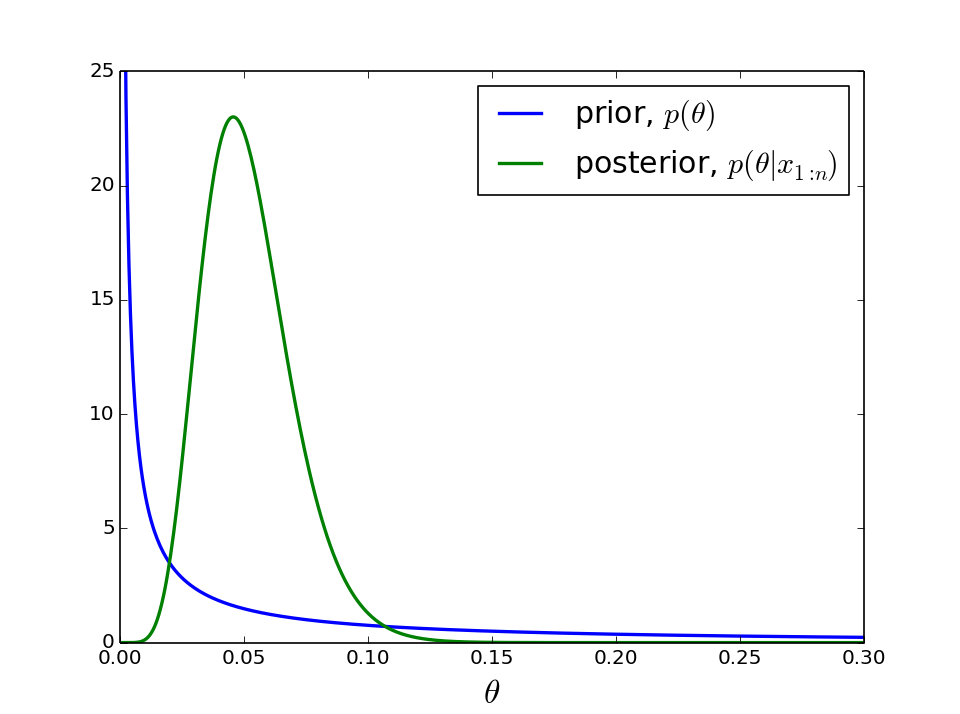
\includegraphics[width=0.7\textwidth]{homework.png}
    % Source: Original work of J. W. Miller.
  \end{center}
  \caption{Prior and posterior densities.}
  \label{figure:posterior}
\end{figure}


\subsection*{Exercise 3}

A minimal requirement for using an Exponential model would be that the data is always positive-valued and continuous (not discrete). However, this is not enough to justify using this model. For any parametric model, it is important that the data can be ``well-fit'' for some choice of parameter values. (For the purposes of this homework, I wouldn't have expected you to know how to assess this yet---but you should learn it now.) Before seeing the data, this can be judged by knowing roughly how the data is generated (see below), and after seeing the data, by conducting tests such as goodness-of-fit or posterior predictive checks (which we will discuss later).

The Exponential distribution has certain special properties (e.g., memorylessness, time between events in a Poisson process, characterization in terms of extreme value theory) that make it well-suited to certain applications. For instance, the ``memorylessness'' property is that if $X\sim\Exp(\theta)$, then for any $s,t\geq 0$,
$$\Pr(X>s+t \mid X>s) = \Pr(X>t).$$
The Poisson process connection is easier to think about (for me at least). If you can have something that is well-characterized by a Poisson process, then the inter-arrival times are i.i.d.\ Exponentials.
In addition to the examples given in Lecture 1, another example would be the time between occurrences of a very rare disease caused by a genetic mutation, such as acromegaly (which often leads to ``gigantism'', see \url{http://en.wikipedia.org/wiki/Gigantism}), if we assume a constant overall birthrate over the period of time of observation.

A simple example of something that would not be well-modeled by a Exponential distribution would be anything that could take negative values or is discrete---e.g., the amount of money you have minus what you owe, or the number of children in a family. An example of something positive-valued that would not be well-fit by an Exponential distribution is the distribution of heights of adult humans.



\subsection*{Exercise 4}

Since $\ell(s,a) =\I(s\neq a)$ then
\begin{align*}
\rho(a,x_{1:n}) & =\E(\ell(S,a)|x_{1:n})\\
& =\E(\I(S\neq a)|x_{1:n})\\
& =\Pr(S\neq a\mid x_{1:n})\\
& =1 - \Pr(S = a\mid x_{1:n}).
\end{align*}
Thus,
$$\argmin_a \rho(a,x_{1:n}) = \argmax_a \Pr(S = a\mid x_{1:n}),$$
that is, the action $a$ that minimizes $\rho(a,x_{1:n})$ is the same as the action $a$ that maximizes the posterior probability $\Pr(S = a\mid x_{1:n})$.


\subsection*{Exercise 5}

Intuitively, the simplest thing that occurs to me is to look at the sample mean $\bar x =\frac{1}{n}\sum_{i = 1}^n x_i$ and see if it is greater than $1/2$. This leads to the decision rule:
$$\delta_1(x_{1:n}) = \I(\bar x>\tfrac{1}{2}). $$

Now, for the Bayes rule. Taking $S = X_{n+1}$ and $a=x_{n+1}$, from Exercise 4 we know that the Bayes procedure is to choose $x_{n+1}$ to maximize $\Pr(X_{n+1}=x_{n+1} \mid x_{1:n})$, i.e., to maximize the posterior predictive, which we know from Lecture 2 is
$$p(x_{n+1}|x_{1:n}) = \frac{a_n^{x_{n+1}} b_n^{1-x_{n+1}}}{a_n + b_n}\I(x_{n+1}\in\{0,1\})$$
where $a_n = a +\sum x_i$ and $b_n = b + n-\sum x_i$.
This gives us the decision rule
$$\delta_2(x_{1:n}) =\I(a_n>b_n),$$
or, after rearranging terms,
$$\delta_2(x_{1:n}) = \I\big(\bar x>\tfrac{1}{2} +\tfrac{b-a}{2 n}\big). $$


\subsection*{Exercise 6}

Yes, for my choice of $\delta_1$ in Exercise 5, they are the same when $a=b$.  Qualitatively speaking, the larger $a$ is relative to $b$, the more the ``balance'' is tilted towards favoring $x_{n+1}=1$ when using the Bayes procedure, compared to the intuitive procedure (and vice versa for $b$ larger than $a$). 

When the difference between $a$ and $b$ is sizable (relative to $n$), the procedure pays less attention to the data and more attention to the prior.  On the other hand, as $n$ grows, the influence of the prior becomes less and less since $\tfrac{b-a}{2 n} \to 0$ as $n\to \infty$.

(Note: A useful and common way of thinking about $a$ and $b$ is as ``pseudo-counts'', that is, as if we had observed $a$ ones and $b$ zeros before the experiment began.)

\subsection*{Exercise 7}

The mean of the Beta distribution $\Beta(a,b)$ is $a/(a+b)$. Thus, the prior mean is $\E(\btheta) = a/(a+b)$. From Lecture 1, the posterior is $\Beta(a_n,b_n)$ where $a_n = a +\sum x_i$ and $b_n = b + n-\sum x_i$. Hence, the posterior mean is 
\begin{align*}
\E(\btheta|x_{1:n}) &= \frac{a_n}{a_n + b_n} \\
& = \frac{a + \sum x_i}{a + b + n} \\
& = \frac{a + b}{a + b + n}\frac{a}{a+b} + \frac{n}{a+b+n}\frac{1}{n}\sum x_i \\
& = (1-t) \E(\btheta) + t \bar x
\end{align*}
with $t = n/(a+b+n)$.

\subsection*{Exercise 8}

See Figure \ref{figure:rho}. See Appendix for source code.

\begin{figure}
  \begin{center}
    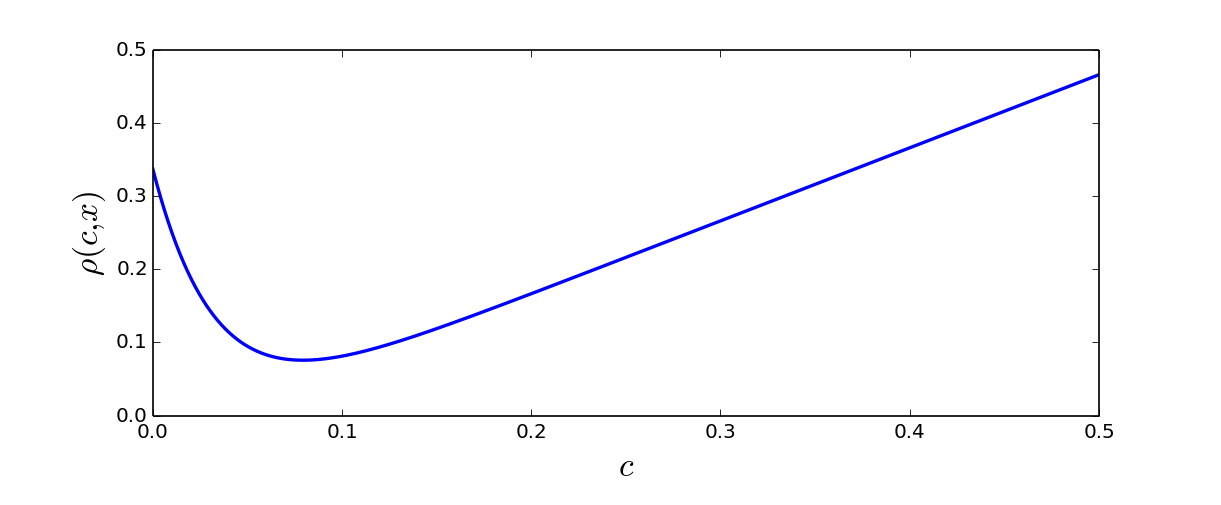
\includegraphics[width=0.85\textwidth]{rho.png}
    % Source: Original work by J. W. Miller.
  \end{center}
  \caption{Posterior expected loss for the disease prevalence example.}
  \label{figure:rho}
\end{figure}

\subsection*{Exercise 9}

A canonical example of this is in medical diagnosis.  Suppose $S$ indicates whether a
certain patient has a certain type of cancer ($S=1$) or not ($S=0$).  A screening test is performed,
yielding data $x$, and from this a decision is made as to whether the patient tests positive or not.  
If a positive diagnosis is made but the patient does not have cancer (``false positive''),
the patient will unnecessarily suffer emotional distress, physical discomfort from further testing,
and monetary costs.
On the other hand, if a negative diagnosis is made but the patient actually does have cancer
(``false negative''), she or he could die prematurely. Due to the asymmetry in these consequences,
the $0-1$ loss is typically not appropriate.  A better loss function would be as follows:
\begin{center}
\begin{tabular}{l r|c|c|}
\multicolumn{2}{r}{} & \multicolumn{2}{c}{Diagnosis} \\
\multicolumn{2}{r}{}
 & \multicolumn{1}{c}{$0$}
 & \multicolumn{1}{c}{$1$} \\
\cline{3-4}
\multirow{2}{*}{Truth} 
   & $0$ & $0$ & $\alpha$ \\
   \cline{3-4}
   & $1$ & $\beta$ & $0$ \\
   \cline{3-4}
\end{tabular}
\end{center}
where $\alpha,\beta>0$ but $\alpha\neq\beta$.  
(Note: This is purely hypothetical, and should not be construed as recommended practice.)









\appendix
\section{Source code in Julia language}

\subsection*{Exercise 2}
\lstinputlisting[language=julia,numbers=none,commentstyle=\tt\color{OliveGreen},firstline=11]{code/homework.jl}

\subsection*{Exercise 8}
\lstinputlisting[language=julia,numbers=none,commentstyle=\tt\color{OliveGreen},firstline=2]{code/rho-mod.jl}


\end{document}






